\documentclass[12pt,a4paper]{article}
\usepackage[latin1]{inputenc}
\usepackage{float}
\usepackage{amsmath}
\usepackage{amsfonts}
\usepackage{amssymb}
\usepackage{graphicx}
\usepackage{fancyhdr}
\usepackage[hidelinks]{hyperref}

\pagestyle{fancy}
\fancyhf{}
\rfoot{Marco Gasperini - Ibrahim El Shemy - Davide Hu}
\title{\textbf{\Huge{HYPERMEDIA WEBSITE PROJECT}} \\ \large Design Document}
\author{Marco Gasperini - 10533178@polimi.it\\ Ibrahim El Shemy - 10491265@polimi.it \\ Davide Hu - 10493858@polimi.it}
\date{A.Y. 2018/2019 ??/??/???? delivery date}

\begin{document}
\maketitle
\newpage
\tableofcontents
\newpage

\section{Abstract}
During the implementation of a Web App the first step is making a document that describes the structure and shows the design model.\\For this purpose we have used the schemes C, L - IDM which show respectively:
\begin{itemize}
\item The conceptual model and the decisions related to it
\item The logical scheme in detail
\end{itemize}

\section{Design-in-the-large}
\subsection{C-IDM}
\begin{figure}[h]
\centering
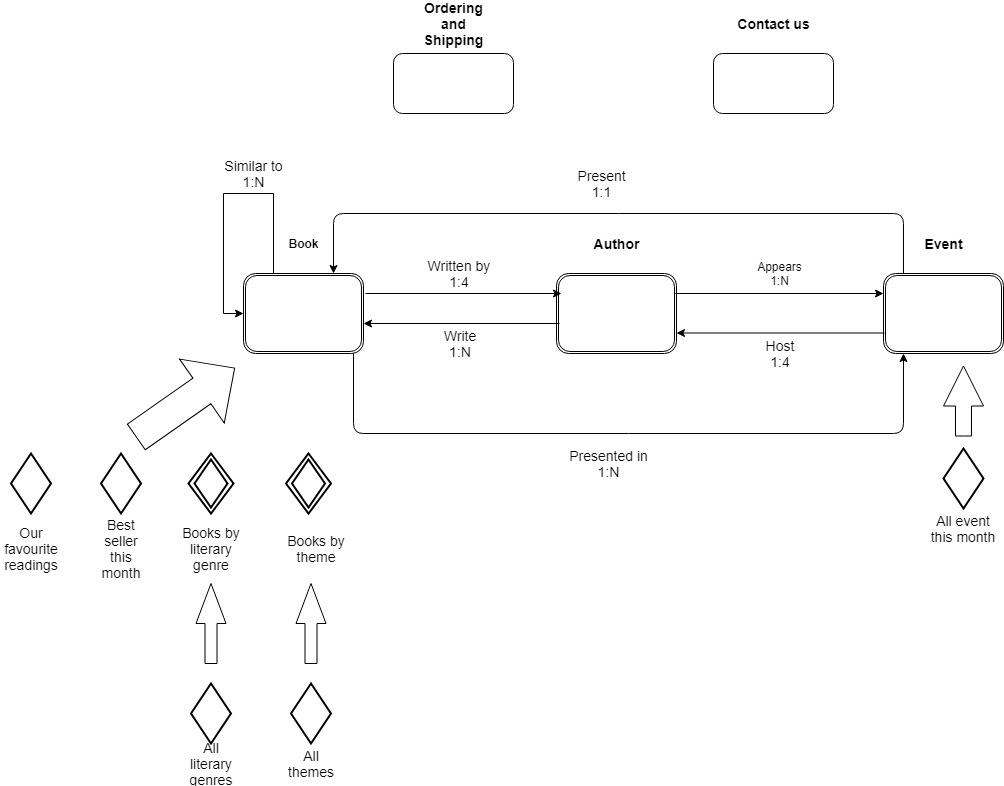
\includegraphics[width=1.0\linewidth]{imm.jpg}
\caption{C-IDM design}
\label{fig:IDM}
\end{figure}

\subsection{L-IDM}
\section{Design-in-the-small}
\section{Design of DB}
\section{Scenarios}
In this section we can find three scenarios with a little description of its and some commented miniaturized screenshots that the user would traverse to execute the scenario.
\subsection{First scenario}
\subsection{Second scenario}
\subsection{Third scenario}
\end{document}